\documentclass{standalone}
\usepackage{tikz}
\usetikzlibrary{patterns, positioning}
\usepackage[sfdefault]{ClearSans} %% option 'sfdefault' activates Clear Sans as the default text font
\usepackage[T1]{fontenc}

\begin{document}
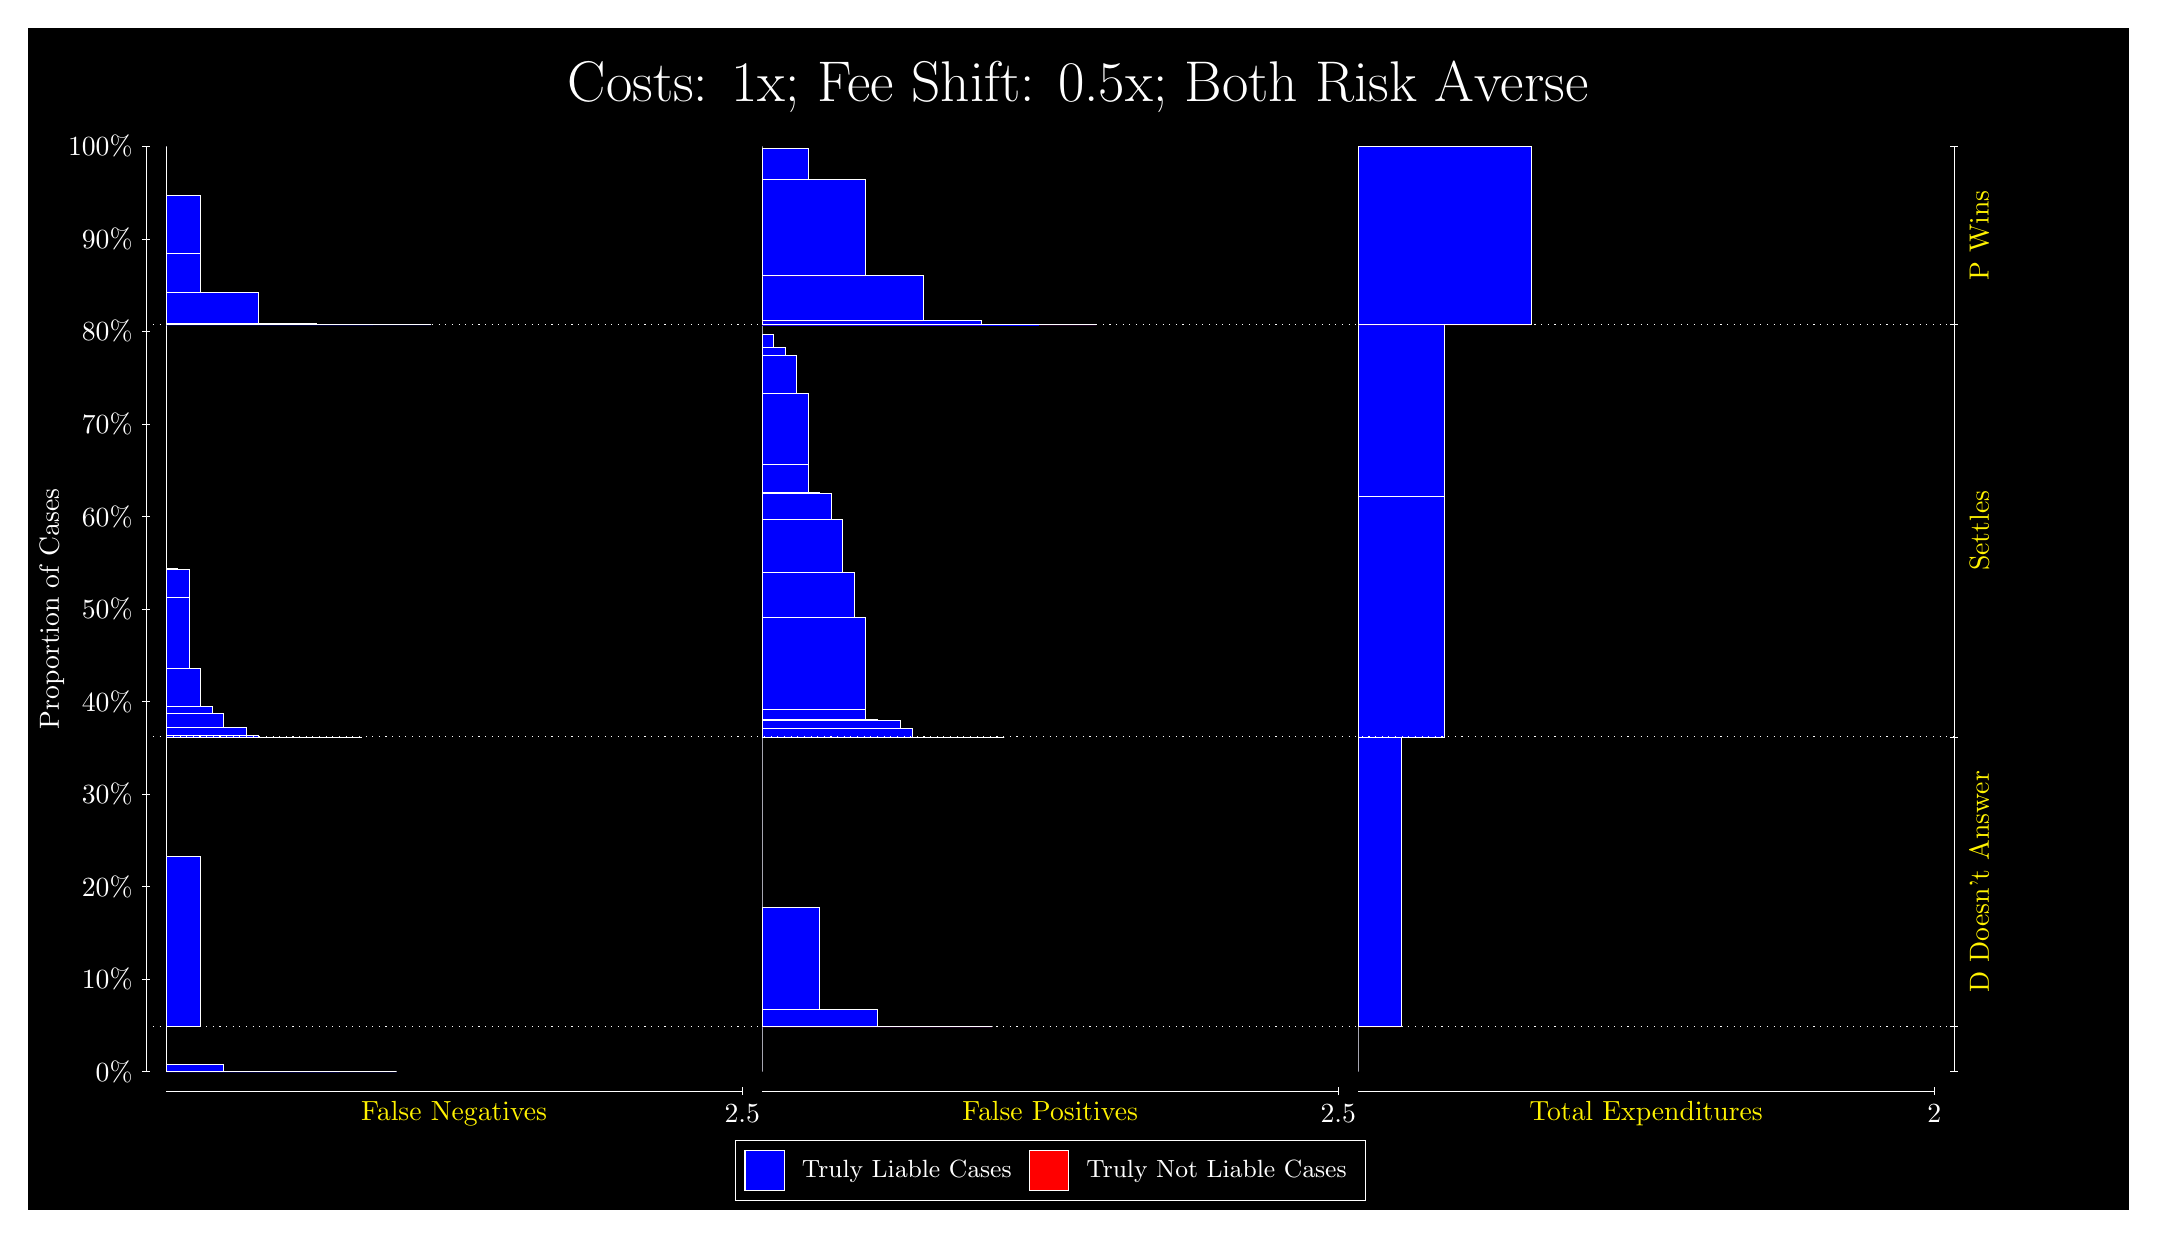
\begin{tikzpicture}
\draw[fill=black] (0,0) rectangle (26.667,15);
\draw[text=white] (0,13.5) rectangle (26.667,15) node[midway] {\huge Costs: 1x; Fee Shift: 0.5x; Both Risk Averse};
\draw[white, very thin] (1.5,1.75) -- (1.5,13.5);
\node[rotate=90, text=white, anchor=center] at (0.3, 7.625) {Proportion of Cases};
\draw[white, very thin] (1.45,1.75) -- (1.55,1.75);
\node[text=white, anchor=east] at (1.45, 1.75) {0\%};
\draw[white, very thin] (1.45,2.925) -- (1.55,2.925);
\node[text=white, anchor=east] at (1.45, 2.925) {10\%};
\draw[white, very thin] (1.45,4.1) -- (1.55,4.1);
\node[text=white, anchor=east] at (1.45, 4.1) {20\%};
\draw[white, very thin] (1.45,5.275) -- (1.55,5.275);
\node[text=white, anchor=east] at (1.45, 5.275) {30\%};
\draw[white, very thin] (1.45,6.45) -- (1.55,6.45);
\node[text=white, anchor=east] at (1.45, 6.45) {40\%};
\draw[white, very thin] (1.45,7.625) -- (1.55,7.625);
\node[text=white, anchor=east] at (1.45, 7.625) {50\%};
\draw[white, very thin] (1.45,8.8) -- (1.55,8.8);
\node[text=white, anchor=east] at (1.45, 8.8) {60\%};
\draw[white, very thin] (1.45,9.975) -- (1.55,9.975);
\node[text=white, anchor=east] at (1.45, 9.975) {70\%};
\draw[white, very thin] (1.45,11.15) -- (1.55,11.15);
\node[text=white, anchor=east] at (1.45, 11.15) {80\%};
\draw[white, very thin] (1.45,12.325) -- (1.55,12.325);
\node[text=white, anchor=east] at (1.45, 12.325) {90\%};
\draw[white, very thin] (1.45,13.5) -- (1.55,13.5);
\node[text=white, anchor=east] at (1.45, 13.5) {100\%};

\draw[white, very thin] (24.457,1.75) -- (24.457,13.5);
\draw[white, very thin] (24.407,1.75) -- (24.507,1.75);
\node[anchor=west] at (24.407, 1.75) {};
\draw[white, very thin] (24.407,2.3201) -- (24.507,2.3201);
\node[anchor=west] at (24.407, 2.3201) {};
\draw[white, very thin] (24.407,5.9998) -- (24.507,5.9998);
\node[anchor=west] at (24.407, 5.9998) {};
\draw[white, very thin] (24.407,11.236) -- (24.507,11.236);
\node[anchor=west] at (24.407, 11.236) {};
\draw[white, very thin] (24.407,13.5) -- (24.507,13.5);
\node[anchor=west] at (24.407, 13.5) {};

\draw[white, very thin, fill=blue] (1.75,1.75) rectangle (4.6775,1.75);
\draw[white, very thin, fill=blue] (1.75,1.75) rectangle (3.9457,1.75);
\draw[white, very thin, fill=blue] (1.75,1.75) rectangle (3.2138,1.7508);
\draw[white, very thin, fill=blue] (1.75,1.7508) rectangle (2.4819,1.8433);
\draw[white, very thin, fill=red] (1.75,1.8433) rectangle (1.75,1.8433);
\draw[white, very thin, fill=blue] (1.75,1.8433) rectangle (1.75,2.3201);
\draw[white, very thin, fill=blue] (1.75,2.3201) rectangle (2.1891,4.4811);
\draw[white, very thin, fill=red] (1.75,4.4811) rectangle (1.75,4.4811);
\draw[white, very thin, fill=blue] (1.75,4.4811) rectangle (1.75,5.9998);
\draw[white, very thin, fill=blue] (1.75,5.9998) rectangle (4.2384,5.9998);
\draw[white, very thin, fill=blue] (1.75,5.9998) rectangle (3.6529,5.9998);
\draw[white, very thin, fill=blue] (1.75,5.9998) rectangle (3.5065,5.9999);
\draw[white, very thin, fill=blue] (1.75,5.9999) rectangle (3.3602,5.9999);
\draw[white, very thin, fill=blue] (1.75,5.9999) rectangle (3.0674,6.0001);
\draw[white, very thin, fill=blue] (1.75,6.0001) rectangle (2.921,6.0151);
\draw[white, very thin, fill=blue] (1.75,6.0151) rectangle (2.7746,6.1268);
\draw[white, very thin, fill=blue] (1.75,6.1268) rectangle (2.6283,6.1273);
\draw[white, very thin, fill=blue] (1.75,6.1273) rectangle (2.4819,6.2939);
\draw[white, very thin, fill=blue] (1.75,6.2939) rectangle (2.3355,6.3898);
\draw[white, very thin, fill=blue] (1.75,6.3898) rectangle (2.1891,6.8687);
\draw[white, very thin, fill=blue] (1.75,6.8687) rectangle (2.0428,7.7778);
\draw[white, very thin, fill=blue] (1.75,7.7778) rectangle (2.0428,8.1287);
\draw[white, very thin, fill=blue] (1.75,8.1287) rectangle (1.8964,8.1411);
\draw[white, very thin, fill=red] (1.75,8.1411) rectangle (1.75,8.1411);
\draw[white, very thin, fill=blue] (1.75,8.1411) rectangle (1.75,11.236);
\draw[white, very thin, fill=blue] (1.75,11.236) rectangle (5.1167,11.236);
\draw[white, very thin, fill=blue] (1.75,11.236) rectangle (4.3848,11.236);
\draw[white, very thin, fill=blue] (1.75,11.236) rectangle (3.6529,11.259);
\draw[white, very thin, fill=blue] (1.75,11.259) rectangle (2.921,11.649);
\draw[white, very thin, fill=blue] (1.75,11.649) rectangle (2.1891,12.144);
\draw[white, very thin, fill=blue] (1.75,12.144) rectangle (2.1891,12.88);
\draw[white, very thin, fill=red] (1.75,12.88) rectangle (1.75,12.88);
\draw[white, very thin, fill=blue] (1.75,12.88) rectangle (1.75,13.5);
\draw[white, very thin, fill=red] (9.3189,1.75) rectangle (9.3189,1.75);
\draw[white, very thin, fill=blue] (9.3189,1.75) rectangle (9.3189,2.3201);
\draw[white, very thin, fill=red] (9.3189,2.3201) rectangle (12.246,2.3201);
\draw[white, very thin, fill=blue] (9.3189,2.3201) rectangle (12.246,2.3201);
\draw[white, very thin, fill=blue] (9.3189,2.3201) rectangle (11.515,2.3219);
\draw[white, very thin, fill=blue] (9.3189,2.3219) rectangle (10.783,2.539);
\draw[white, very thin, fill=blue] (9.3189,2.539) rectangle (10.051,3.8388);
\draw[white, very thin, fill=blue] (9.3189,3.8388) rectangle (9.3189,5.9998);
\draw[white, very thin, fill=red] (9.3189,5.9998) rectangle (12.393,5.9998);
\draw[white, very thin, fill=blue] (9.3189,5.9998) rectangle (12.393,5.9998);
\draw[white, very thin, fill=red] (9.3189,5.9998) rectangle (12.1,5.9998);
\draw[white, very thin, fill=blue] (9.3189,5.9998) rectangle (12.1,5.9998);
\draw[white, very thin, fill=red] (9.3189,5.9998) rectangle (11.807,5.9998);
\draw[white, very thin, fill=blue] (9.3189,5.9998) rectangle (11.807,6);
\draw[white, very thin, fill=blue] (9.3189,6) rectangle (11.661,6);
\draw[white, very thin, fill=red] (9.3189,6) rectangle (11.515,6);
\draw[white, very thin, fill=blue] (9.3189,6) rectangle (11.515,6);
\draw[white, very thin, fill=blue] (9.3189,6) rectangle (11.368,6.0007);
\draw[white, very thin, fill=red] (9.3189,6.0007) rectangle (11.222,6.0007);
\draw[white, very thin, fill=blue] (9.3189,6.0007) rectangle (11.222,6.1124);
\draw[white, very thin, fill=blue] (9.3189,6.1124) rectangle (11.075,6.2049);
\draw[white, very thin, fill=blue] (9.3189,6.2049) rectangle (10.929,6.2167);
\draw[white, very thin, fill=blue] (9.3189,6.2167) rectangle (10.783,6.2173);
\draw[white, very thin, fill=blue] (9.3189,6.2173) rectangle (10.636,6.3488);
\draw[white, very thin, fill=red] (9.3189,6.3488) rectangle (10.636,6.3488);
\draw[white, very thin, fill=blue] (9.3189,6.3488) rectangle (10.636,7.521);
\draw[white, very thin, fill=blue] (9.3189,7.521) rectangle (10.49,8.0923);
\draw[white, very thin, fill=blue] (9.3189,8.0923) rectangle (10.344,8.7695);
\draw[white, very thin, fill=blue] (9.3189,8.7695) rectangle (10.197,9.095);
\draw[white, very thin, fill=blue] (9.3189,9.095) rectangle (10.051,9.1074);
\draw[white, very thin, fill=blue] (9.3189,9.1074) rectangle (9.9044,9.4583);
\draw[white, very thin, fill=blue] (9.3189,9.4583) rectangle (9.9044,10.367);
\draw[white, very thin, fill=blue] (9.3189,10.367) rectangle (9.758,10.846);
\draw[white, very thin, fill=blue] (9.3189,10.846) rectangle (9.6116,10.942);
\draw[white, very thin, fill=blue] (9.3189,10.942) rectangle (9.4652,11.109);
\draw[white, very thin, fill=blue] (9.3189,11.109) rectangle (9.3189,11.236);
\draw[white, very thin, fill=red] (9.3189,11.236) rectangle (13.564,11.236);
\draw[white, very thin, fill=blue] (9.3189,11.236) rectangle (13.564,11.236);
\draw[white, very thin, fill=red] (9.3189,11.236) rectangle (12.832,11.236);
\draw[white, very thin, fill=blue] (9.3189,11.236) rectangle (12.832,11.237);
\draw[white, very thin, fill=red] (9.3189,11.237) rectangle (12.1,11.237);
\draw[white, very thin, fill=blue] (9.3189,11.237) rectangle (12.1,11.286);
\draw[white, very thin, fill=red] (9.3189,11.286) rectangle (11.368,11.286);
\draw[white, very thin, fill=blue] (9.3189,11.286) rectangle (11.368,11.856);
\draw[white, very thin, fill=red] (9.3189,11.856) rectangle (10.636,11.856);
\draw[white, very thin, fill=blue] (9.3189,11.856) rectangle (10.636,13.087);
\draw[white, very thin, fill=blue] (9.3189,13.087) rectangle (9.9044,13.478);
\draw[white, very thin, fill=blue] (9.3189,13.478) rectangle (9.3189,13.5);
\draw[white, very thin, fill=red] (16.888,1.75) rectangle (16.888,1.75);
\draw[white, very thin, fill=blue] (16.888,1.75) rectangle (16.888,2.3201);
\draw[white, very thin, fill=red] (16.888,2.3201) rectangle (17.437,2.3201);
\draw[white, very thin, fill=blue] (16.888,2.3201) rectangle (17.437,5.9998);
\draw[white, very thin, fill=red] (16.888,5.9998) rectangle (17.986,5.9998);
\draw[white, very thin, fill=blue] (16.888,5.9998) rectangle (17.986,9.0616);
\draw[white, very thin, fill=red] (16.888,9.0616) rectangle (17.986,9.0616);
\draw[white, very thin, fill=blue] (16.888,9.0616) rectangle (17.986,11.236);
\draw[white, very thin, fill=red] (16.888,11.236) rectangle (19.083,11.236);
\draw[white, very thin, fill=blue] (16.888,11.236) rectangle (19.083,13.5);
\draw[white, dotted] (1.5,2.3201) -- (24.457,2.3201);
\draw[white, dotted] (1.5,5.9998) -- (24.457,5.9998);
\draw[white, dotted] (1.5,11.236) -- (24.457,11.236);
\draw[white, very thin] (1.75,1.5) -- (9.0689,1.5);
\node[text=yellow, anchor=north] at (5.4094, 1.5) {False Negatives};
\draw[white, very thin] (9.0689,1.45) -- (9.0689,1.55);
\node[text=white, anchor=north] at (9.0689, 1.45) {2.5};

\draw[white, very thin] (9.3189,1.5) -- (16.638,1.5);
\node[text=yellow, anchor=north] at (12.978, 1.5) {False Positives};
\draw[white, very thin] (16.638,1.45) -- (16.638,1.55);
\node[text=white, anchor=north] at (16.638, 1.45) {2.5};

\draw[white, very thin] (16.888,1.5) -- (24.207,1.5);
\node[text=yellow, anchor=north] at (20.547, 1.5) {Total Expenditures};
\draw[white, very thin] (24.207,1.45) -- (24.207,1.55);
\node[text=white, anchor=north] at (24.207, 1.45) {2};


\node[text=yellow, centered, rotate=90] at (24.777, 4.1599) {D Doesn't Answer};
\node[text=yellow, centered, rotate=90] at (24.777, 8.6181) {Settles};
\node[text=yellow, centered, rotate=90] at (24.777, 12.368) {P Wins};

\draw (12.978300999999998,1.5) node[draw=none] (baseCoordinate) {};
\begin{scope}[align=center]
        \matrix[scale=0.5, draw=white, below=0.5cm of baseCoordinate, nodes={draw}, column sep=0.1cm]{
            \node[rectangle, draw, minimum width=0.5cm, minimum height=0.5cm, fill=blue] {}; &
            \node[draw=none, font=\small, text=white] (B) {Truly Liable Cases}; &
            \node[rectangle, draw, minimum width=0.5cm, minimum height=0.5cm, fill=red] {}; &
            \node[draw=none, font=\small, text=white] (B) {Truly Not Liable Cases}; \\
            };
\end{scope}

\end{tikzpicture}
\end{document}